% ============================================================================
% DÉFINITION DU COURS 01 : INGÉNIERIE SYSTÈME
% ============================================================================

\titlehead{Thomas Lusseau - SII en ATS}
\title[Introduction à l'ingénierie système]{Introduction à l'ingénierie système}
\author[TL]{Thomas Lusseau}
\date{\today}

\TLCourseCoverSetup
  {\repStyle/FondPoly.png}
  {images/image3.png}
  {Cycle 1 : Analyser, expérimenter et\\ communiquer sur les systèmes pluritechnologiques}
  {Introduction à l'ingénierie système}
  {Lycée Robert Doisneau - ATS}
  {Thomas Lusseau}

\TLCourseCoverContents{%
  \TLCourseContentsLine{1.1}{Systèmes, besoin et cycle de vie}{sec:is-systeme}
  \TLCourseContentsLine{1.2}{Système souhaité, simulé et réel}{sec:is-ecarts}
  \TLCourseContentsLine{1.3}{Démarche d'ingénierie système}{sec:is-demarche}
  \TLCourseContentsLine{1.4}{Exigences, vérification et validation}{sec:is-exigences}
  \TLCourseContentsLine{1.5}{Langage et diagrammes SysML}{sec:is-sysml}
  \TLCourseContentsLine{1.6}{Architecture fonctionnelle}{sec:is-architecture-fonctionnelle}
  \TLCourseContentsLine{1.7}{Exercices du chapitre}{sec:is-exercices}
}

\TLCourseFooter
\TLCourseCover
\markboth{Introduction à l'ingénierie système}{Introduction à l'ingénierie système}

\AtBeginEnvironment{corrige}{\small}
\livrettrue
\collefalse

\TLStartCourseChapter{1}{Introduction à l'ingénierie système}{chap:ingenierie-systeme}

\begin{savoirs}
\begin{itemize}
  \item définition, typologie, frontière et cycle de vie d'un système ;
  \item démarche d'ingénierie système et gestion des exigences ;
  \item vérification, validation, traçabilité et gestion des interfaces ;
  \item rôle des principaux diagrammes SysML ;
  \item architecture fonctionnelle, chaîne d'information et chaîne d'énergie.
\end{itemize}
\end{savoirs}

\begin{savoirfaire}
\begin{itemize}
  \item analyser un besoin et identifier les parties prenantes ;
  \item formuler une exigence mesurable et définir sa méthode de preuve ;
  \item lire et compléter un diagramme de contexte, d'exigences, BDD ou IBD ;
  \item relier les fonctions aux solutions techniques et aux flux ;
  \item comparer système souhaité, système simulé et système réel.
\end{itemize}
\end{savoirfaire}

% ==========================================================================
% COURS 01 -- PARTIE A : SYSTÈMES, BESOIN ET CYCLE DE VIE
% ==========================================================================

\section{Mise en situation}\label{sec:is-mise-situation}

La réussite d'un produit ne dépend pas seulement de la qualité de chacun de ses composants. Elle dépend surtout de la capacité à comprendre le besoin, à prendre en compte l'environnement, à organiser les interfaces et à vérifier que la solution finale satisfait les parties prenantes.

\begin{ISapplication}[title={Une solution technique peut être localement correcte et globalement inadaptée}]
Lors du repêchage d'un véhicule, une grue insuffisamment stabilisée peut basculer malgré le bon fonctionnement de son treuil. Le problème ne vient pas nécessairement d'un composant défaillant, mais d'une mauvaise prise en compte du système complet : charge, portée, stabilité, sol, opérateur et scénario d'utilisation.
\end{ISapplication}

\begin{center}
\begin{minipage}[c]{.48\linewidth}
\centering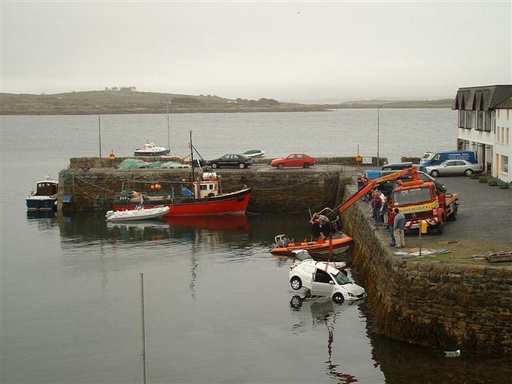
\includegraphics[width=\linewidth,height=.25\textheight,keepaspectratio]{images/image5.jpeg}
\end{minipage}\hfill
\begin{minipage}[c]{.48\linewidth}
\centering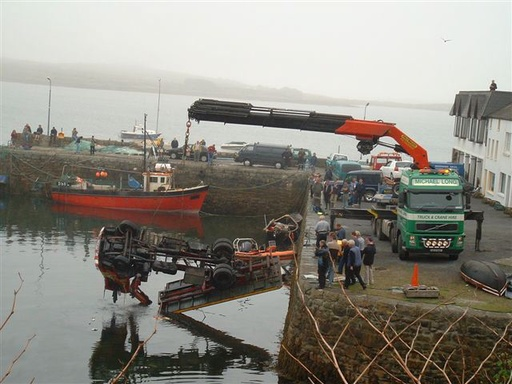
\includegraphics[width=\linewidth,height=.25\textheight,keepaspectratio]{images/image8.jpeg}
\end{minipage}
\end{center}

Les erreurs de conception apparaissent aussi lorsque les interfaces avec l'existant sont mal maîtrisées : gabarit d'un train et dimensions des quais, logiciel et réseau, véhicule et réglementation, produit et maintenance.

\section{Définir un système}\label{sec:is-systeme}

\begin{ISdefinition}
Un \textbf{système} est un ensemble d'éléments en interaction, organisé pour atteindre un ou plusieurs résultats quantifiables en termes de performance.
\end{ISdefinition}

Un système possède :
\begin{itemize}
  \item une finalité et des fonctions ;
  \item une frontière qui distingue le système de son environnement ;
  \item des constituants organisés selon une architecture ;
  \item des interfaces par lesquelles circulent matière, énergie et information ;
  \item des performances mesurables.
\end{itemize}

\ISSystemeBoiteNoire

\subsection{Systèmes naturels et artificiels}

Les systèmes naturels existent indépendamment d'une intention de conception : système solaire, organisme vivant ou écosystème. Les systèmes artificiels sont créés ou transformés par l'être humain pour répondre à un besoin.

En sciences industrielles, on étudie principalement des systèmes artificiels pluritechnologiques associant mécanique, électronique, informatique, automatique, énergie et communication.

\subsection{Frontière et environnement}

La frontière dépend de la question posée. Pour étudier l'autonomie d'un véhicule, la batterie appartient au système. Pour étudier la fabrication de cette batterie, les procédés industriels et les matières premières deviennent eux-mêmes des sous-systèmes étudiés.

\ISContexte

\begin{ISattention}
Une frontière mal définie conduit à oublier une interface ou à attribuer au système une performance qui dépend en réalité d'un élément extérieur. La frontière doit toujours être explicitée.
\end{ISattention}

\section{Besoin, fonction et solution}\label{sec:is-besoin}

\subsection{Besoin}

Le besoin décrit ce qu'attend une partie prenante sans imposer prématurément une solution technique. Il doit être formulé du point de vue du service rendu.

Exemple : « permettre à une personne à mobilité réduite de franchir un dénivelé en sécurité » est un besoin. « installer un moteur de 500 W » est déjà une solution.

\subsection{Fonctions de service et contraintes}

Une fonction de service exprime une action utile entre le système et son environnement. Une contrainte limite la liberté du concepteur : sécurité, norme, masse, encombrement, coût, environnement ou maintenance.

Une formulation efficace utilise un verbe à l'infinitif et un complément :
\begin{itemize}
  \item déplacer une charge ;
  \item informer l'utilisateur ;
  \item résister à l'humidité ;
  \item limiter les nuisances sonores.
\end{itemize}

\begin{ISmethode}[title={Formuler une exigence fonctionnelle}]
\begin{enumerate}
  \item Identifier la partie prenante concernée.
  \item Décrire le service attendu sans citer de solution.
  \item Associer un critère mesurable.
  \item Fixer un niveau et une flexibilité ou tolérance.
  \item Préciser le scénario de vérification.
\end{enumerate}
\end{ISmethode}

\section{Trois représentations du système}\label{sec:is-ecarts}

Au cours d'une démarche de conception, on distingue :
\begin{description}
  \item[Système souhaité :] défini par le besoin, les exigences et le cahier des charges ;
  \item[Système simulé :] représenté par des modèles numériques ou analytiques ;
  \item[Système réel :] prototype ou produit effectivement réalisé et mesuré.
\end{description}

\ISTriangleSystemes

Les trois écarts fondamentaux sont :
\begin{itemize}
  \item écart entre souhaité et simulé : qualité du modèle et choix de conception ;
  \item écart entre simulé et réel : incertitudes, hypothèses et réalisation ;
  \item écart entre réel et souhaité : conformité du produit au besoin.
\end{itemize}

La démarche expérimentale sert à quantifier ces écarts et à améliorer soit le produit, soit le modèle, soit la formulation des exigences.

\section{Cycle de vie d'un système}\label{sec:is-cycle-vie}

Le cycle de vie couvre l'ensemble des étapes depuis l'expression du besoin jusqu'au retrait de service :
\begin{enumerate}
  \item analyse du besoin et faisabilité ;
  \item spécification et conception ;
  \item réalisation et intégration ;
  \item vérification et validation ;
  \item production, exploitation et maintenance ;
  \item évolution, réemploi, recyclage ou élimination.
\end{enumerate}

La prise en compte du cycle de vie dès la conception évite de déplacer les problèmes vers la fabrication, l'utilisation, la maintenance ou la fin de vie.

\subsection{Approche environnementale}

L'analyse de cycle de vie évalue les consommations de ressources et les impacts environnementaux sur toutes les étapes. Elle évite qu'une amélioration locale ne crée un impact plus important ailleurs.

Les principales familles d'indicateurs concernent :
\begin{itemize}
  \item consommation d'énergie et de ressources non renouvelables ;
  \item émissions de gaz à effet de serre ;
  \item acidification, eutrophisation et toxicité ;
  \item déchets, bruit, occupation des sols et consommation d'eau.
\end{itemize}

\begin{ISapplication}[title={Éco-conception}]
Réduire la masse d'un produit peut diminuer l'énergie consommée pendant son usage, mais rendre le recyclage plus complexe si des matériaux composites indissociables sont utilisés. L'évaluation doit porter sur le cycle complet.
\end{ISapplication}

% ==========================================================================
% COURS 01 -- PARTIE B : INGÉNIERIE SYSTÈME ET EXIGENCES
% ==========================================================================

\section{L'approche d'ingénierie système}\label{sec:is-demarche}

L'ingénierie système organise les activités nécessaires à la conception, à la réalisation et à l'exploitation de systèmes complexes. Elle vise à maîtriser simultanément les besoins, les exigences, les interfaces, les risques, les modèles et les preuves de conformité.

\begin{ISdefinition}
L'\textbf{ingénierie système} est une démarche interdisciplinaire qui transforme un besoin en une solution cohérente sur l'ensemble du cycle de vie, en assurant la traçabilité entre attentes, exigences, architecture, réalisation, vérification et validation.
\end{ISdefinition}

Elle ne remplace pas les disciplines techniques. Elle permet de les coordonner : mécanique, électronique, informatique, automatique, énergétique, ergonomie, sûreté, industrialisation et maintenance.

\subsection{Parties prenantes}

Une partie prenante est une personne, une organisation ou un système concerné par le produit. Elle peut exprimer un besoin, imposer une contrainte, utiliser, maintenir, financer, fabriquer ou contrôler le système.

Exemples : utilisateur final, exploitant, mainteneur, fabricant, organisme de contrôle, riverain, assureur, autorité réglementaire ou système connecté.

\begin{ISmethode}[title={Identifier les parties prenantes}]
Pour chaque phase du cycle de vie, se demander :
\begin{enumerate}
  \item qui utilise ou subit les effets du système ;
  \item qui fournit matière, énergie ou information ;
  \item qui fabrique, transporte, installe, maintient ou recycle ;
  \item qui autorise, contrôle ou finance ;
  \item quels autres systèmes échangent avec lui.
\end{enumerate}
\end{ISmethode}

\subsection{Démarche descendante et démarche ascendante}

La démarche \textbf{descendante} part de la mission et des exigences pour définir les fonctions, puis les sous-systèmes et les composants. La démarche \textbf{ascendante} intègre les composants réalisés, vérifie les sous-systèmes puis valide le système complet.

\ISCycleEnV

Le cycle en V met en correspondance les activités de définition à gauche et les activités de preuve à droite :
\begin{itemize}
  \item les composants sont testés ;
  \item les sous-systèmes sont intégrés et vérifiés ;
  \item le système complet est validé vis-à-vis du besoin.
\end{itemize}

\begin{ISattention}
Le cycle en V ne signifie pas que toutes les décisions sont figées dès le début. Les revues, prototypes et essais produisent des retours qui conduisent à corriger les exigences ou l'architecture. La traçabilité permet de maîtriser ces évolutions.
\end{ISattention}

\section{Exigences et cahier des charges}\label{sec:is-exigences}

\begin{ISdefinition}
Une \textbf{exigence} est une caractéristique ou une capacité que le système doit posséder pour satisfaire un besoin, respecter une règle ou permettre une vérification.
\end{ISdefinition}

Une exigence de qualité doit être :
\begin{itemize}
  \item nécessaire et justifiée ;
  \item claire et non ambiguë ;
  \item réalisable ;
  \item mesurable ou vérifiable ;
  \item cohérente avec les autres exigences ;
  \item identifiée de manière unique ;
  \item reliée à sa source et à une méthode de preuve.
\end{itemize}

\subsection{Attributs d'une exigence}

Une exigence comporte généralement :
\begin{description}
  \item[Identifiant :] code unique et stable ;
  \item[Texte :] formulation du résultat attendu ;
  \item[Source :] partie prenante, norme ou décision à l'origine ;
  \item[Critère et niveau :] grandeur mesurable et valeur attendue ;
  \item[Flexibilité :] tolérance, priorité ou marge de négociation ;
  \item[Méthode de vérification :] inspection, analyse, démonstration ou essai ;
  \item[Statut :] proposée, approuvée, modifiée ou vérifiée.
\end{description}

\ISDiagrammeExigences

\subsection{Hiérarchie et dérivation}

Une exigence globale peut être décomposée en exigences plus précises. La dérivation doit conserver l'intention initiale et permettre de justifier chaque exigence de niveau inférieur.

Exemple : l'exigence « transporter une personne en sécurité » peut être dérivée en masse admissible, vitesse maximale, distance d'arrêt, résistance mécanique, disponibilité de l'arrêt d'urgence et conformité réglementaire.

\subsection{Traçabilité}

La traçabilité relie :
\[
\text{besoin}\longrightarrow\text{exigence}\longrightarrow\text{fonction}
\longrightarrow\text{solution}\longrightarrow\text{preuve}.
\]

Elle permet de répondre à quatre questions :
\begin{itemize}
  \item pourquoi cet élément existe-t-il ;
  \item quelle exigence satisfait-il ;
  \item quelles exigences seraient affectées par sa modification ;
  \item où se trouve la preuve de conformité.
\end{itemize}

\begin{ISapplication}[title={Matrice de traçabilité simplifiée}]
\begin{center}
\begin{tabularx}{.92\linewidth}{>{\bfseries}p{.18\linewidth}X X}
\toprule
Exigence & Élément de solution & Preuve prévue \\
\midrule
REQ-1 Masse $\geq100$ kg & structure et actionneur & calcul puis essai de charge \\
REQ-2 Vitesse $\leq1{,}5$ m/s & variateur et loi de commande & mesure chronométrique \\
REQ-3 Arrêt $<0{,}5$ s & frein et arrêt d'urgence & essai instrumenté \\
\bottomrule
\end{tabularx}
\end{center}
\end{ISapplication}

\section{Vérification et validation}\label{sec:is-verification-validation}

\begin{ISdefinition}[title={Vérification}]
La \textbf{vérification} répond à la question : « le système a-t-il été réalisé conformément à ses spécifications ? »
\end{ISdefinition}

\begin{ISdefinition}[title={Validation}]
La \textbf{validation} répond à la question : « le système réalisé répond-il réellement au besoin des parties prenantes dans son contexte d'utilisation ? »
\end{ISdefinition}

Une exigence peut être vérifiée par :
\begin{itemize}
  \item \textbf{inspection} : examen visuel, dimension ou document ;
  \item \textbf{analyse} : calcul ou simulation ;
  \item \textbf{démonstration} : observation d'un fonctionnement ;
  \item \textbf{essai} : mesure selon un protocole défini.
\end{itemize}

\begin{ISattention}
Un produit peut être conforme à toutes ses spécifications et pourtant ne pas satisfaire l'utilisateur si le besoin a été mal compris. La vérification ne remplace donc pas la validation.
\end{ISattention}

\section{Architecture, interfaces et compromis}\label{sec:is-architecture}

L'architecture répartit les fonctions et les exigences entre des sous-systèmes. Elle décrit leur organisation et leurs interfaces.

Une interface peut transmettre :
\begin{itemize}
  \item de la matière : fluide, pièce, charge ;
  \item de l'énergie : électrique, mécanique, hydraulique, thermique ;
  \item de l'information : mesure, ordre, état ou donnée réseau.
\end{itemize}

Les interfaces sont souvent à l'origine des difficultés d'intégration. Elles doivent préciser les grandeurs échangées, les unités, les connecteurs, les protocoles, les tolérances et les responsabilités.

\subsection{Compromis de conception}

Les exigences peuvent être antagonistes :
\begin{itemize}
  \item diminuer la masse peut augmenter le coût ;
  \item augmenter la vitesse peut réduire la sécurité ou l'autonomie ;
  \item accroître la précision peut nécessiter des capteurs plus coûteux ;
  \item rendre un produit démontable peut augmenter son encombrement.
\end{itemize}

Le choix d'une architecture résulte d'un compromis explicite, justifié par des critères pondérés et par les priorités du projet.

\section{Risques, configuration et évolutions}\label{sec:is-risques}

La gestion des risques identifie les événements susceptibles d'empêcher l'atteinte des objectifs. Un risque est souvent caractérisé par sa probabilité et sa gravité.

Les actions possibles sont : éviter, réduire, transférer ou accepter le risque. Les risques critiques doivent être associés à des mesures de prévention, de détection et de réduction des conséquences.

La gestion de configuration garantit que les documents, modèles, logiciels et composants utilisés correspondent à une version identifiée. Toute modification doit être analysée, approuvée et répercutée sur les éléments liés.

\begin{ISmethode}[title={Analyser une modification}]
\begin{enumerate}
  \item Identifier la raison et la version concernée.
  \item Rechercher les exigences et interfaces liées.
  \item Évaluer les conséquences techniques, économiques et calendaires.
  \item Mettre à jour modèles, plans, code, essais et documentation.
  \item Vérifier puis valider à nouveau les éléments affectés.
\end{enumerate}
\end{ISmethode}

% ==========================================================================
% COURS 01 -- PARTIE C : SYSML ET ARCHITECTURE FONCTIONNELLE
% ==========================================================================

\section{Le langage SysML}\label{sec:is-sysml}

SysML est un langage graphique de modélisation destiné aux systèmes complexes. Il permet de représenter plusieurs vues complémentaires d'un même système sans prétendre remplacer les modèles de calcul propres à chaque discipline.

\begin{ISdefinition}
Un \textbf{modèle SysML} est un ensemble cohérent d'objets, de relations et de diagrammes décrivant les exigences, le comportement, la structure et les contraintes d'un système.
\end{ISdefinition}

Un diagramme est une vue partielle du modèle. Une information importante ne doit pas être dupliquée sans lien : elle doit être définie une fois puis réutilisée dans plusieurs vues.

\subsection{Familles de diagrammes}

Les diagrammes couramment utilisés en sciences industrielles sont :

\begin{center}
\begin{tabularx}{\linewidth}{>{\bfseries}p{.25\linewidth}p{.13\linewidth}X}
\toprule
Diagramme & Acronyme & Rôle principal \\
\midrule
Exigences & RD & hiérarchiser, dériver et tracer les exigences \\
Cas d'utilisation & UCD & décrire les services attendus par les acteurs \\
Séquence & SD & ordonner les échanges entre acteurs et composants \\
États-transitions & SMD & décrire les états et événements d'un système \\
Activités & AD & représenter un processus, des actions et des flux \\
Définition de blocs & BDD & décrire la composition et la typologie des blocs \\
Blocs internes & IBD & représenter les ports, connecteurs et flux internes \\
Paramétrique & PD & relier des paramètres par des équations ou contraintes \\
\bottomrule
\end{tabularx}
\end{center}

\begin{ISattention}
Un diagramme SysML n'est pas un dessin libre. Chaque symbole et chaque relation ont une signification. La lisibilité ne doit pas conduire à inventer une notation ambiguë.
\end{ISattention}

\section{Diagramme de contexte et cas d'utilisation}\label{sec:is-contexte-usecase}

Le diagramme de contexte représente le système et les éléments extérieurs qui interagissent avec lui pendant une phase de vie donnée.

\ISContexte

Un cas d'utilisation exprime un service rendu à un acteur. Son nom est formulé avec un verbe à l'infinitif et un complément : « transporter une personne », « enregistrer une vidéo », « signaler un défaut ».

Les acteurs principaux sont ceux qui bénéficient directement du service. Les acteurs secondaires fournissent une ressource, une information ou une contrainte.

\begin{ISmethode}[title={Construire une vue de contexte}]
\begin{enumerate}
  \item Choisir une phase de vie et définir la frontière.
  \item Placer le système au centre.
  \item Recenser acteurs, milieux physiques, sources d'énergie et systèmes voisins.
  \item Nommer les échanges de matière, d'énergie et d'information.
  \item Déduire les services et contraintes associés.
\end{enumerate}
\end{ISmethode}

\section{Diagramme d'exigences}\label{sec:is-rd}

Le diagramme d'exigences rassemble des objets portant un identifiant et un texte. Les principales relations sont :
\begin{description}
  \item[Contenance :] une exigence en contient d'autres ;
  \item[«deriveReqt» :] une exigence est dérivée d'une exigence plus globale ;
  \item[«refine» :] un élément précise une exigence ;
  \item[«satisfy» :] un bloc ou une solution satisfait une exigence ;
  \item[«verify» :] un cas de test vérifie une exigence ;
  \item[«trace» :] lien de traçabilité générique.
\end{description}

\ISDiagrammeExigences

Le diagramme ne remplace pas la spécification textuelle complète. Il rend visibles la hiérarchie et les liens, tandis que les attributs détaillés restent associés aux objets du modèle.

\section{Diagrammes de structure : BDD et IBD}\label{sec:is-bdd-ibd}

\ISBDDIBD

\subsection{Diagramme de définition de blocs}

Le BDD décrit les types de blocs, leurs propriétés et leurs relations. Une composition signifie qu'un bloc est constitué de parties dont la durée de vie dépend du bloc parent.

Il permet notamment de représenter :
\begin{itemize}
  \item la décomposition système, sous-systèmes, composants ;
  \item les valeurs et paramètres ;
  \item les associations et généralisations ;
  \item les contraintes affectées à un type de bloc.
\end{itemize}

\subsection{Diagramme de blocs internes}

L'IBD décrit l'intérieur d'une instance de bloc. Il montre les parties, les ports, les connecteurs et les flux échangés.

Les ports précisent les interfaces. Les flux sont nommés et peuvent être typés : tension, couple, information numérique, débit, position ou température.

\begin{ISapplication}[title={Chaîne d'un axe motorisé}]
Dans un axe électrique, le contrôleur transmet une commande au variateur, le variateur alimente le moteur, le moteur fournit un couple au transmetteur, et un capteur renvoie une mesure de position. Le BDD décrit les composants ; l'IBD décrit leurs échanges.
\end{ISapplication}

\section{Diagrammes de comportement}\label{sec:is-comportement}

\subsection{Diagramme de séquence}

Le diagramme de séquence représente les échanges entre lignes de vie dans l'ordre chronologique. Il est adapté aux scénarios : démarrage, authentification, cycle nominal ou gestion d'un défaut.

Un message synchrone bloque l'émetteur jusqu'au retour. Un message asynchrone permet à l'émetteur de poursuivre son activité.

\subsection{Diagramme d'activités}

Le diagramme d'activités décrit un enchaînement d'actions et de flux. Il comporte des nœuds de décision, de fusion, de parallélisation et de synchronisation.

Il convient à la description d'un processus de fonctionnement ou d'une procédure de maintenance, sans nécessairement attribuer chaque action à un composant précis.

\subsection{Diagramme d'états-transitions}

Le diagramme d'états-transitions décrit les états successifs d'un bloc et les événements qui provoquent les transitions.

Une transition peut comporter :
\[
\text{événement}\ [\text{garde}]\ /\ \text{effet}.
\]

Les activités \texttt{entry}, \texttt{do} et \texttt{exit} précisent les actions à l'entrée, pendant et à la sortie d'un état.

\section{Architecture fonctionnelle}\label{sec:is-architecture-fonctionnelle}

L'architecture fonctionnelle organise les fonctions nécessaires à la réalisation du service. Elle se place avant le choix détaillé des composants et facilite la recherche de solutions alternatives.

\subsection{Fonction globale et fonctions techniques}

La fonction globale décrit la transformation principale réalisée par le système. Elle est décomposée en fonctions techniques plus élémentaires jusqu'à un niveau permettant d'identifier des solutions.

Une décomposition fonctionnelle doit être :
\begin{itemize}
  \item complète par rapport aux exigences ;
  \item indépendante autant que possible des solutions ;
  \item cohérente avec les flux entrants et sortants ;
  \item traçable vers les composants qui réaliseront les fonctions.
\end{itemize}

\subsection{Chaîne d'information et chaîne d'énergie}

\ISChaineFonctionnelle

La chaîne d'information assure généralement :
\begin{itemize}
  \item \textbf{acquérir} les consignes et grandeurs physiques ;
  \item \textbf{traiter} les informations et décider ;
  \item \textbf{communiquer} vers l'utilisateur ou d'autres systèmes.
\end{itemize}

La chaîne d'énergie assure :
\begin{itemize}
  \item \textbf{alimenter} le système ;
  \item \textbf{distribuer} ou moduler l'énergie ;
  \item \textbf{convertir} l'énergie en énergie mécanique utile ;
  \item \textbf{transmettre} et adapter le mouvement ou l'effort ;
  \item \textbf{agir} sur la matière d'œuvre.
\end{itemize}

\begin{ISattention}
Les deux chaînes ne sont pas indépendantes. Les ordres issus du traitement commandent la distribution d'énergie, et les capteurs observent la chaîne d'énergie ou l'effecteur.
\end{ISattention}

\subsection{Diagramme FAST}

Le FAST organise les fonctions en répondant aux questions « pourquoi ? » vers la gauche et « comment ? » vers la droite. Les fonctions nécessaires simultanément sont placées verticalement.

Il aide à distinguer la finalité, les fonctions de service et les fonctions techniques, puis à rechercher plusieurs principes de solution.

\begin{ISmethode}[title={Passer du besoin à l'architecture}]
\begin{enumerate}
  \item Définir la mission, la frontière et les scénarios.
  \item Formaliser les exigences mesurables.
  \item Identifier les flux à transformer.
  \item Décomposer la fonction globale.
  \item Regrouper les fonctions en sous-systèmes cohérents.
  \item Définir les interfaces et allouer les exigences.
  \item Comparer plusieurs architectures avant de choisir les composants.
\end{enumerate}
\end{ISmethode}

\section{Exploitation des modèles en SII}\label{sec:is-exploitation}

Les diagrammes SysML servent de fil directeur aux études disciplinaires. Ils permettent de localiser le sous-système étudié, d'identifier ses entrées et sorties, de retrouver l'exigence à vérifier et de replacer un calcul dans l'architecture complète.

Une étude de mécanique, d'automatique ou d'électronique doit donc se conclure par une comparaison quantitative avec l'exigence correspondante.

\begin{center}
\begin{tabularx}{\linewidth}{>{\bfseries}p{.23\linewidth}X X}
\toprule
Étape & Question & Support possible \\
\midrule
Analyser & quel service et quelles contraintes ? & contexte, UCD, RD \\
Modéliser & quelles grandeurs et quelles relations ? & BDD, IBD, PD, modèles physiques \\
Simuler & quelles performances prévues ? & modèle numérique et scénarios \\
Expérimenter & quelles performances réelles ? & protocole, mesures et incertitudes \\
Conclure & l'exigence est-elle satisfaite ? & matrice de traçabilité et rapport \\
\bottomrule
\end{tabularx}
\end{center}

\section{Sources}\label{sec:is-sources}

Ce chapitre reprend les contenus du cours d'analyse fonctionnelle et d'introduction à l'ingénierie système, en harmonisant la démarche, les diagrammes SysML et l'architecture fonctionnelle avec le framework commun des cours de SII en ATS.

% ==========================================================================
% COURS 01 -- EXERCICES
% ==========================================================================

\section{Exercices du chapitre}\label{sec:is-exercices}

\begin{TLExercise}{Exercice 1 -- Repêchage d'un véhicule}
Un camion-grue doit relever une voiture tombée dans un port. La première tentative provoque le basculement du camion ; un second véhicule équipé de stabilisateurs est nécessaire.
\begin{enumerate}
  \item Formuler le besoin sans imposer de solution technique.
  \item Définir la frontière du système étudié.
  \item Identifier au moins six éléments de l'environnement.
  \item Proposer quatre exigences mesurables liées à la sécurité et à la performance.
  \item Distinguer les causes relevant d'un composant et celles relevant de l'intégration du système.
\end{enumerate}
\end{TLExercise}

\begin{TLExercise}{Exercice 2 -- Compatibilité d'un train avec les quais}
Une nouvelle rame est plus large afin d'améliorer le confort, mais certaines infrastructures anciennes ne respectent pas un gabarit uniforme.
\begin{enumerate}
  \item Identifier les parties prenantes et les interfaces critiques.
  \item Écrire une exigence de compatibilité vérifiable.
  \item Proposer une méthode de vérification avant la fabrication en série.
  \item Expliquer la différence entre vérification de la rame et validation du service de transport.
\end{enumerate}
\end{TLExercise}

\begin{TLExercise}{Exercice 3 -- Drone de loisir}
Un drone doit permettre à un utilisateur de filmer une scène en extérieur.
\begin{enumerate}
  \item Formuler la mission du système.
  \item Construire la liste des acteurs d'un diagramme de contexte.
  \item Proposer cinq cas d'utilisation formulés par un verbe et un complément.
  \item Écrire six exigences dont deux contraintes réglementaires ou environnementales.
  \item Associer à chaque exigence une méthode de preuve.
\end{enumerate}
\end{TLExercise}

\begin{TLExercise}{Exercice 4 -- Micro-ondes}
On étudie un four à micro-ondes domestique pendant sa phase d'utilisation.
\begin{enumerate}
  \item Définir la matière d'œuvre entrante et sortante.
  \item Énoncer la fonction globale.
  \item Identifier les flux de matière, d'énergie et d'information.
  \item Répartir les fonctions dans les chaînes d'information et d'énergie.
  \item Citer trois autres phases de vie nécessitant un contexte différent.
\end{enumerate}
\end{TLExercise}

\begin{TLExercise}{Exercice 5 -- Diagramme d'exigences}
La mission d'une plateforme élévatrice est de transporter une personne entre deux niveaux. Les exigences initiales sont : charge minimale de 120 kg, vitesse inférieure à 0,15 m/s, arrêt d'urgence en moins de 0,4 s et niveau sonore inférieur à 65 dB(A).
\begin{enumerate}
  \item Attribuer un identifiant à chaque exigence.
  \item Distinguer exigences fonctionnelles et contraintes.
  \item Proposer une exigence globale dont elles dérivent.
  \item Associer à chacune un critère, un niveau, une tolérance et une méthode de vérification.
  \item Représenter les relations «deriveReqt», «satisfy» et «verify».
\end{enumerate}
\end{TLExercise}

\begin{TLExercise}{Exercice 6 -- BDD et IBD d'un axe motorisé}
Un axe comprend un contrôleur, un variateur, un moteur, un réducteur, un chariot et un capteur de position.
\begin{enumerate}
  \item Proposer la décomposition du système dans un BDD.
  \item Identifier les relations de composition.
  \item Décrire les flux échangés dans un IBD.
  \item Préciser la nature et l'unité de chaque flux.
  \item Localiser les interfaces qui devraient faire l'objet d'une spécification détaillée.
\end{enumerate}
\end{TLExercise}

\begin{TLExercise}{Exercice 7 -- Scénario de démarrage}
Un robot mobile reçoit un ordre de départ, vérifie la fermeture de son capot, initialise ses capteurs, libère son frein puis commence à se déplacer. En cas de défaut, il signale une alarme et reste immobile.
\begin{enumerate}
  \item Représenter le scénario sous forme de diagramme de séquence.
  \item Proposer un diagramme d'activités avec décision et branche de défaut.
  \item Définir les états principaux d'un diagramme d'états-transitions.
  \item Écrire deux transitions sous la forme événement [garde] / effet.
\end{enumerate}
\end{TLExercise}

\begin{TLExercise}{Exercice 8 -- Système souhaité, simulé et réel}
La simulation d'un vérin prévoit une course de 500 mm en 4,5 s. Le cahier des charges impose une course d'au moins 490 mm en moins de 5 s. Les mesures donnent 486 mm en 4,8 s.
\begin{enumerate}
  \item Identifier les données relevant des systèmes souhaité, simulé et réel.
  \item Quantifier les trois écarts pertinents.
  \item Conclure sur chaque exigence.
  \item Proposer deux causes possibles de l'écart simulation-réel.
  \item Indiquer si le modèle, le produit ou l'exigence doit être révisé.
\end{enumerate}
\end{TLExercise}

\begin{TLExercise}{Exercice 9 -- Cycle de vie et éco-conception}
Deux solutions de carter sont comparées : aluminium recyclable plus lourd, ou composite plus léger mais difficile à séparer en fin de vie.
\begin{enumerate}
  \item Lister les étapes du cycle de vie à comparer.
  \item Identifier les flux et impacts principaux de chaque solution.
  \item Expliquer pourquoi la seule masse en phase d'usage ne suffit pas pour conclure.
  \item Proposer des indicateurs environnementaux et économiques.
  \item Définir les données supplémentaires nécessaires à la décision.
\end{enumerate}
\end{TLExercise}

\begin{TLExercise}{Exercice 10 -- Modification d'une batterie}
La capacité de la batterie d'un robot est augmentée de 40\%. La nouvelle batterie est plus lourde, plus volumineuse et délivre une tension nominale différente.
\begin{enumerate}
  \item Identifier les exigences susceptibles d'être affectées.
  \item Recenser les interfaces à vérifier.
  \item Proposer une analyse des impacts sur structure, motorisation, autonomie, sécurité et logiciel.
  \item Lister les documents et modèles à mettre à jour.
  \item Définir les essais de non-régression nécessaires.
\end{enumerate}
\end{TLExercise}

\begin{TLExercise}{Exercice 11 -- Architecture fonctionnelle d'un portail automatique}
Un portail doit détecter une demande, vérifier l'absence d'obstacle, déverrouiller, déplacer le vantail, ralentir en fin de course et informer l'utilisateur.
\begin{enumerate}
  \item Formuler la fonction globale.
  \item Construire une décomposition fonctionnelle de type FAST.
  \item Répartir les fonctions dans les chaînes d'information et d'énergie.
  \item Associer à chaque fonction une ou plusieurs solutions techniques possibles.
  \item Identifier les boucles d'information liées à la sécurité.
\end{enumerate}
\end{TLExercise}

\begin{TLExercise}{Exercice 12 -- Étude de synthèse : véhicule autonome}
Un véhicule autonome urbain doit transporter quatre personnes sur un trajet prédéfini, respecter le code de la route et fonctionner par tous les temps raisonnables.
\begin{enumerate}
  \item Identifier les principales parties prenantes et construire le contexte d'utilisation.
  \item Proposer les cas d'utilisation principaux et secondaires.
  \item Rédiger dix exigences mesurables couvrant performance, sécurité, environnement et maintenance.
  \item Définir une architecture fonctionnelle et les flux principaux.
  \item Proposer une décomposition en sous-systèmes pour un BDD.
  \item Décrire un scénario nominal et un scénario de défaillance.
  \item Construire une matrice reliant exigences, sous-systèmes et méthodes de preuve.
  \item Expliquer comment les systèmes souhaité, simulé et réel seront comparés.
\end{enumerate}
\end{TLExercise}

